\section{Circuito de gabinete central}

Se comenzó el desarrollo del proyecto con el diseño del gabinete central. El mismo debe ser capaz de alimentar los módulos, con \SI{12}{\volt} de corriente continua y \SI{48}{\volt} de corriente alterna. Además, debe contar con el microcontrolador encargado de manejar el sistema completo y los conectores para la comunicación con los módulos y con los periféricos necesarios para la interfaz de usuario.

\subsection{Alimentación}

Para la alimentación, se compró una fuente conmutada de \SI{12}{\volt} de corriente continua, \SI{5}{\ampere} máximo de salida (\SI{60}{\watt}), con entrada \SI{220}{\volt} de corriente alterna. Además, se compró un transformador de corriente alterna de entrada \SI{220}{\volt} y salida \SI{48}{\volt}, \SI{1}{\ampere} máximo de salida (\SI{48}{\voltampere}). 

\subsection{Control}

Para el control del sistema en general se decidió utilizar el microcontrolador Espressif ESP32-S3, \parencite{esp32s3}, por su versatilidad compacta y robustez funcional: dispone de una gran cantidad de entradas/salidas configurables y dos conversores analógico-digitales de 12 bits.

\subsection{Interfaz de usuario}

Para la interfaz de usuario, se decidió utilizar un \textit{display} LCD TFT de \SI{2.8}{''} con comunicación SPI y resolución de 240x320 píxeles; y un \textit{encoder} rotativo para navegación.

\subsection{Circuito}

En la figura \cref{fig:gabinete:diagrama}, se observa un diagrama en bloque del circuito diseñado. Para la comunicación entre el gabinete central y los módulos, se utiliza un cable plano soldado directamente a la placa del gabinete central, con un conector PCIe x4 hembra en el otro extremo.

\begin{figure}[H]
    \centering
    \resizebox{0.65\textwidth}{!}{
        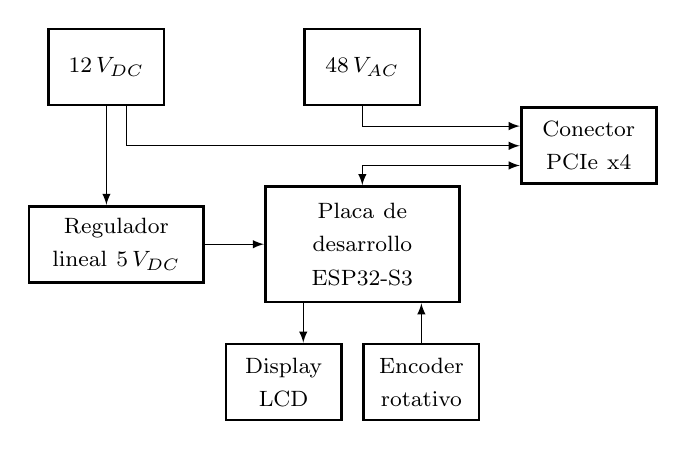
\begin{tikzpicture}
            % Paths, nodes and wires:
            \node[shape=rectangle, draw, line width=1pt, minimum width=1.465cm, minimum height=0.965cm] at (1.75, 6){} node[anchor=center, align=center, text width=1.077cm, inner sep=6pt] at (1.75, 6){\footnotesize $12\, V_{DC}$};
            \node[shape=rectangle, draw, line width=1pt, minimum width=1.465cm, minimum height=0.965cm] at (5, 6){} node[anchor=center, align=center, text width=1.077cm, inner sep=6pt] at (5, 6){\footnotesize $48\, V_{AC}$};
            \node[shape=rectangle, draw, line width=1pt, minimum width=1.715cm, minimum height=0.965cm] at (7.875, 5){} node[anchor=center, align=center, text width=1.327cm, inner sep=6pt] at (7.875, 5){\footnotesize Conector PCIe x4};
            \node[shape=rectangle, draw, line width=1pt, minimum width=2.465cm, minimum height=1.465cm] at (5, 3.75){} node[anchor=center, align=center, text width=2.077cm, inner sep=6pt] at (5, 3.75){\footnotesize Placa de desarrollo ESP32-S3};
            \node[shape=rectangle, draw, line width=1pt, minimum width=1.465cm, minimum height=0.965cm] at (4, 2){} node[anchor=center, align=center, text width=1.077cm, inner sep=6pt] at (4, 2){\footnotesize Display LCD};
            \node[shape=rectangle, draw, line width=1pt, minimum width=1.465cm, minimum height=0.965cm] at (5.75, 2){} node[anchor=center, align=center, text width=1.077cm, inner sep=6pt] at (5.75, 2){\footnotesize Encoder rotativo};
            \node[shape=rectangle, draw, line width=1pt, minimum width=2.215cm, minimum height=0.965cm] at (1.875, 3.75){} node[anchor=center, align=center, text width=1.827cm, inner sep=6pt] at (1.875, 3.75){\footnotesize Regulador lineal $5\,V_{DC}$};
            \draw[-latex] (5, 5.5) -- (5, 5.25) -- (7, 5.25);
            \draw[-latex] (2, 5.5) -| (2, 5) -- (7, 5);
            \draw[-latex] (1.75, 5.5) -- (1.75, 4.25);
            \draw[latex-latex] (5, 4.5) |- (7, 4.75);
            \draw[-latex] (5.75, 2.5) -| (5.75, 3);
            \draw[-latex] (3, 3.75) -- (3.75, 3.75);
            \draw[-latex] (4.25, 3) -| (4.25, 2.5);
        \end{tikzpicture}
    }
    \caption{Diagrama en bloques del circuito del gabinete central.}
    \label{fig:gabinete:diagrama}
\end{figure}

Una vez diseñado el circuito de la placa del gabinete central, se procede a diseñar los modelos del mismo, así como de los demás componentes del proyecto.